\section {Library}
\label{sec:library}
 
\subsection{Goals}
\label{sec:goals}

The goal of the library is to provide a set of classes that simplify programming in SCOOP. 
Specifically, we want to provide implementations for common concurrency patterns like the worker pool.
The result should be a new Eiffel library similar to the standard concurrency libraries in Java \cite{web:java-concurrency} or C\# \cite{web:ms-tpl}.

The library was developed with the following design goals:

\begin{description}
 \item [Safety]\label{item:safety} Avoid common SCOOP pitfalls like deadlocks, starvation of a processor or unintentional lock passing.
 \item [Convenience]\label{item:convenience} Shield the user from having to write many little ``wrappers'', i.e. features that just lock an object for a single separate call.
 \item [Performance]\label{item:performance} Reduce the overhead of thread creation, especially for code that deals with a lot of small separate objects.
\end{description}

\subsection{Concepts}

This section describes two core concepts of the library: Import and Separate Proxies.
The import concept deals with the problem of how to pass data from one processor to another.
It is useful to achieve the performance and to some extent the safety design goal in Section \ref{sec:goals}.

The Separate Proxy \patternref{SP} is a pattern to hide separate references behind a proxy object.
It provides a solution to the convenience design goal.

\subsubsection{Import}
\label{sec:concepts:import}
% Describe how to use it, i.e. generic parameter and importer objects, and the fact that you can select between import and no import.

The import concept is a central part of the library.
It was developed to let users choose between two object passing strategies, namely the Data Processor and the Import approach (see Section \ref{sec:object-migration}).

The main class is \lstinline!CP_IMPORT_STRATEGY!, which has the simple interface:

\begin{lstlisting}[language=OOSC2Eiffel, captionpos=b, caption={The deferred class CP\_IMPORT\_STRATEGY.}]
deferred class interface
  CP_IMPORT_STRATEGY [G]

feature -- Status report

  is_importable (object: separate G): BOOLEAN
      -- Is `object' importable?

feature -- Duplication

  import (object: separate G): separate G
      -- Import `object'.
    require
      importable: is_importable (object)

end
\end{lstlisting}

%\lstinputlisting [firstline=7] {../../library/import/cp_import_strategy.e}

The class has two descendants.
\lstinline!CP_NO_IMPORTER [G]! can be used for the Data Processor strategy. 
It just perform a reference copy of the object.
The class \lstinline!CP_IMPORTER [G]! on the other hand narrows the return type of \lstinline!import! to a non-separate \lstinline!G!, meaning that it actually performs an import.

As there's no general-purpose import available in SCOOP at the moment users have to implement their own import features for every class that needs this facility.
Descendants of \lstinline!CP_IMPORTER! simplify this task and provide predefined implementations for some standard classes such as \lstinline!STRING!.
Those mechanisms are described in detail in Section \ref{sec:modules:import}.

Components that want to make use of the import mechanism need an instance of \lstinline!CP_IMPORT_STRATEGY! on the same processor.
There are several ways how this object can be supplied to a library component.
The most obvious solution - passing it as an argument in a constructor - has a big drawback in the SCOOP world:
It is impossible to instantiate the component on a separate processor without having to write an extra factory class.

A better solution is to exploit the constrained genericity mechanism in Eiffel.
A component that needs to import objects has to declare an additional generic argument for the import strategy.
A user can then decide on the precise semantics of the import strategy by just declaring the right type.

The constraint placed on the generic argument is that it needs to be a descendant of \lstinline!CP_IMPORT_STRATEGY! and that it needs to declare \lstinline!default_create! as a creation procedure.
The latter is not a big restriction in practice, as there are usually no attributes in an importer anyway.

A typical class header of a component using the import concept looks like this:
\begin{lstlisting}[language=OOSC2Eiffel, captionpos=b, caption={An example component with import.}]
class BUFFER [G, IMPORTER -> 
          CP_IMPORT_STRATEGY [G] create default_create end]

feature -- Access

  item: like {IMPORTER}.import

end
\end{lstlisting}

This small code sample shows another neat little feature of Eiffel.
The \lstinline!like! statement fixes the type based on the chosen import strategy, i.e. \lstinline!separate G! for \lstinline!CP_NO_IMPORTER! and non-separate for descendants of \lstinline!CP_IMPORTER!.
This makes the handling of imported objects a lot easier.

\subsubsection{Separate Proxy}
\label{sec:separate-proxy}

The Separate Proxy pattern \patternref{SP} simplifies access to a separate reference by providing a processor-local proxy object wich forwards all requests to the actual object.
The main advantage is that clients don't need to write extra ``wrapper'' feature to control the separate object.
It is applied to all classes in the library which are meant to be shared among processors, i.e. which are usually accessed through a separate reference.

The pattern consists of three classes:
\begin{description}
 \item [Protégé] The actual business class whose objects are usually shared.
 \item [Helper] A class that provides helper functions to access a separate protégé.
  The helper class is usually ending on \lstinline!_UTILS!.
 \item [Proxy] A proxy class with a similar interface as the protégé class, usually ending on \lstinline!_PROXY!.
    The proxy forwards every call to its protégé, using the helper class.
\end{description}

It is possible to add a fourth, deferred class that just defines a common interface for the protégé and the proxy.
There's an inconsistency however: 
All preconditions in the protégé class that reference \lstinline!Current! (explicitly or implicitly) need to be weakened (i.e. \lstinline!require else True!) in the proxy, and turned into wait conditions in the helper class.
Furthermore, not all features in the business class may be necessary in the proxy, and the proxy itself may add some more features such as compound actions.

\begin{figure}[ht]
\label{fig:separate-proxy}
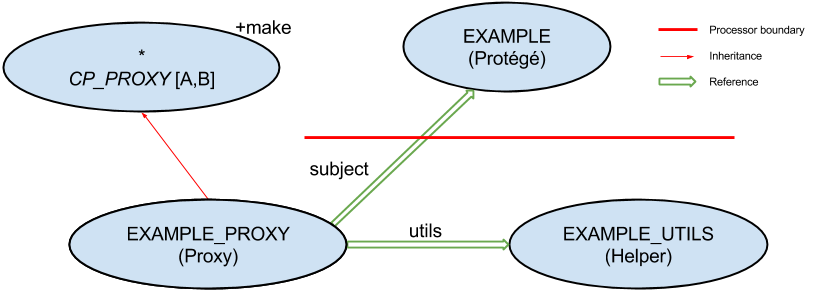
\includegraphics[width=\textwidth]{resources/separate_proxy.png}
\caption{The class relations in the Separate Proxy pattern.}
\end{figure}

Unfortunately this pattern cannot be turned into a reusable module, because it is highly dependent on the precise interface of the protégé class.
There is some support in the library however: 
\lstinline!CP_PROXY! defines a creation procedure and the attributes \lstinline!subject! for a separate protégé object and \lstinline!utils! for a helper object.

Appendix \ref{sec:howto-separate-proxy} provides a general recipe on how to implement a separate proxy for an arbitrary protégé class.

\subsection {Module overview}
\label{sec:module-overview}
% Describe available modules, which patterns they're implementing, and which modules they depend upon.
The library consists of several modules which implement some of the patterns described in the overview (Section \ref{sec:pattern_overview}).
The source code of the library is available on GitHub \cite{web:repository}.
All file locations in the following section are relative to the root directory of the repository.

One of the most basic modules is the import module in \dir{library/import}.
It implements the Import \patternref{IMP} pattern  and is at the same time one of the core concepts of the library.

The queue module in \dir{library/queue} implements the Prdocuer / Consumer \patternref{P/C} pattern.
It depends on the import module.

The process module in \dir{library/process} provides skeleton classes for objects with a main loop.
It provides implementations for the Active Object \patternref{AO}, Asynchronous Self-Call \patternref{ASC} and Timer: Periodic \patternref{TP} patterns.

The worker pool module in \dir{library/worker\_pool} implements the Worker Pool \patternref{WP} pattern.
It uses the import, queue and process module.

The directory \dir{library/promise} contains the promise module.
This module provides classes to monitor and interact with an asynchronous operation.

The executor module resides in \dir{library/executor} and provides an implementation to the Executor Framework \patternref{EF}, 
a specialized worker pool and part of the implementation to the Future pattern \patternref{FUT}.

The implementation of the future pattern is highly intertwined with other parts of the library.
It makes use of the promise, executor and worker pool modules and introduces only two classes on its own:
\lstinline!CP_COMPUTATION! and \lstinline!CP_FUTURE_EXECUTOR_PROXY!.

The class \lstinline!CP_DELAYED_TASK! in \dir{libary/util} implements the Timer: Invoke Later pattern \patternref{TIL}.
The same directory also contains the class \lstinline!CP_EVENT!, which implements the Publish / Subscribe pattern \patternref{P/S} in SCOOP.

